%File: formatting-instruction.tex
\documentclass[letterpaper]{article}
\usepackage{aaai}
\usepackage{times}
\usepackage{helvet}
\usepackage{courier}
\usepackage{graphicx}
\usepackage{hyperref}
\frenchspacing
\setlength{\pdfpagewidth}{8.5in}
\setlength{\pdfpageheight}{11in}
\pdfinfo{
/Title (Insert Your Title Here)
/Author (Put All Your Authors Here, Separated by Commas)}
\setcounter{secnumdepth}{0}  
 \begin{document}
% The file aaai.sty is the style file for AAAI Press 
% proceedings, working notes, and technical reports.
%
\title{Intelligent System \\For Music Generation Deep Learning {}}
\author{\\
\textbf{Aiswarya Siby} (110091664)  (sibya@uwindsor.ca)\\
\textbf{Akhil Punchavallil Sivankuttan}  (110091575) 
 (punchav@uwindsor.ca)\\
\textbf{Jess Joseph Benny}  (110059554)  (bennyj@uwindsor.ca)\\
}
\maketitle
\begin{abstract}
\begin{quote}
Learning music is considered a scarce skill among humans. Humans are perfect at determining whether a piece of music is good or not, but the ability to create soothing music needs years of lessons, practice and experience. So using computers to generate new music pieces is always considered challenging. The increased popularity of deep learning networks for generating images and animations also extended to music generation. In this project, we are creating a music-generation model which consists of a combination of Generative-Adversarial Networks and Recurrent Neural Networks. The project is an extension of MuseGAN, a machine-learning model that uses GANs to generate new music. The project is trained using GiantMIDI-Piano, which contains 10854 piano rolls from 2786 composers from around the globe. The trained model will then be used to generate not just single-instrument music but also can be used to create multitrack music using python libraries such as music21 and midi2audio. 
\end{quote}
\textbf{Keywords - \textit{Music Generation, LSTM, GAN, Deep Learning, Recurrent Neural Network}}
\end{abstract}

\section{Introduction}
Music can be thought of as the culmination of vocal and instrumental sound and has already become an important part of our life and history. Each day sees further growth in the music industry. These songs need a tonne of work, despite the fact that more and more musicians are creating new music. It takes exceptional skills to recognize and differentiate between music from different sources. They apply several ideas, including rhythm, pattern, and pitch control, to create music. In addition to new compositions, technological advancements also play a role in the history of music. Although the process of composing music is difficult, one might become more accustomed to it with the aid of AI. There is tremendous growth in AI and people are more than ever interested in creating artificial intelligence. Music creation is a challenging task even for human minds, so creating soothing sounds through technology would be a great advancement. The process of making music can be streamlined and sped up by automating some of the steps. Automated music makes it possible for musicians to write melodies that can be developed into full-fledged soundtracks in addition to allowing on-musicians to generate music. The sector has been the subject of research for many years. Even though musicians have access to a variety of programmes and resources, those without a musical education haven't seen much progress in the field.

Artificial intelligence for music use neural networks, which are very vast collections of computer components that attempt to simulate how the brain functions. Deep generative neural networks can be effectively trained using generative adversarial networks. The project uses a generative adversarial model that can handle continuous sequential input by instructing it a library of classical music. In recent years, generative neural networks have dominated artistic activities like image creation and photo editing. Another area where these deep learning networks are beginning to have an impact is music production. The suggested method generates music that looks to have been composed by a person using LSTM and GAN neural networks. By considering the notes and chords found in MIDI files as discrete sequential data, it was possible to train these two models and use them to produce wholly new MIDI files.

There is plenty of research regarding the usage of Generative Adversarial Networks for music generation. We are trying to extend the existing project "MuseGAN: Multi-Track Sequential Generative Adversarial Networks for Symbolic Music Generation and Accompaniment" by Hao-Wen Dong et al. The authors of MuseGAN believe that introducing Recurrent Neural Network units to GANs could help the model understand temporal relationships between patterns in a piece of music. We will extend MuseGAN by combining the network with one popularly used RNN unit called Long Short-Term Memory. Things we accomplished by completing this project include

\begin{itemize}
    \item Understand how GANs and RNNs generate new sequence by learning from already existing data
    \item Understand how Recurrent Neural Networks can learn patterns from temporal data
    \item Adding LSTM units to GAN architecture
    \item Train proposed model on GiantMIDI-Piano dataset, which consists of MIDI files of  10854 piano rolls compositions from 2786 composers
    \item Using the trained model to generate new patterns and employing python libraries such as Midi2audio, Music21 to create audio files for the generated music pattern
\end{itemize}

\section{Related Works}

\subsection{MuseGAN}

In their article "MuseGAN: Multi-track Sequential Generative Adversarial Networks for Symbolic Music Generation and Accompaniment," Hao-Wen Dong and colleagues present a three-model framework for multi-track music generation using generative adversarial networks \cite{b2}. Jamming Model, Composer Model, and Hybrid Model are the three models that make up the three-model framework. According to the author, their model was the first to produce polyphonic or multi-track music. For the purpose of representing and training multi-track music, the author offers the idea of multiple-track piano-roll representation. A binary-valued matrix, similar to a scorecard, is used in a piano roll to represent the existence of notes across several time steps. A multiple-track piano roll is a set of piano rolls that may be played on many instruments. Two networks, the discriminator and the generator make up the most generative adversarial networks. 

The generator part of a GAN learns to create fictitious data by taking feedback from the discriminator into account. The power to convince the discriminator that its output is real is gained. A single-channel musical composition is created by a number of independently operating generators in the jamming model, which then receives feedback from various discriminators. One generator produces a multi-channel piano roll for the composer model's single discriminator, which serves as feedback. Ideas from the Composer and Jamming models are combined in the hybrid model. It produces intra-track music using M number of generators. M songs are being evaluated by a single discriminator alone. The Lakh MIDI dataset, which includes roughly 176K piano rolls, was the source of the experimentation data. The author contends that their findings can serve as a starting point for additional research in the field of music creation, even though the music created by machines using these models is not musically calming in comparison to what people make. Research in the future might look into ways to improve the music's calming qualities.

\subsection{Binary Neurons for Polyphonic Music generation}
In their study, "Convolutional Generative Adversarial Networks with Binary Neurons for Polyphonic Music Generations" Hao-Wen Dong and Yi-Hsuan Yang suggest a model that uses binary neurons that can create binary values piano rolls rather than real-values piano roll sequences\cite{b1}. Real-valued piano rolls are produced by existing models, according to the authors, and these rolls need to be processed further using techniques like Hard Thresholding (HT) and Bernoulli Sampling. Added to the generator in the suggested architecture is a refiner network. In order to binarize real-value piano rolls, the refiner and discriminator must first be trained simultaneously. The generator and discriminator are pre-trained in this process. Values are produced in binary by binary neurons.

In this paper, the author discussed two different forms of binary neurons: deterministic binary neurons, which have hard thresholding activation functions, and stochastic binary neurons, which binarize input using a probability function. Refiners are made up of M private networks that convert outputs with actual values into binary. The author creates a refiner with several leftover units in the suggested way. The research use a subset of the Lakh Pianoroll Dataset as the training data. The cleansed subset contains 13,746 phrases drawn from 2,291 songs from which they randomly select six four-bar phrases from each song. This 8-track piano roll dataset is used to train the model. The implementation of a separate HT and BS refiner network, according to the author, produces better outcomes. In order to achieve temporal linkages, further work for this paper will include the addition of recurrent layers to the model.

\subsection{JamBot: Music Theory Aware Chord Based Generation of Polyphonic Music with LSTMs}

The paper Music Theory Aware Chord Based Generation of Polyphonic Music using LSTMs proposes a novel approach for LSTM-based polyphonic music production \cite{b4}. The suggested process creates music in two steps. The chord progression is predicted by LSTM using a chord first embedding. A second LSTM uses the projected chord progression to produce polyphonic music after that. The music is characterized by few disruptive notes and a pleasing harmonic sound. It has a specific long-term structure similar to the type of music that would be played during a jam session by musicians. Researchers can show that the procedure is sound from a music theory perspective by evaluating the learned chord embeddings. The circle of fifths, a vital tool in music theory, was intriguingly extracted from the dataset by the simple model. The algorithm was trained using the lakh MIDI dataset, which had 100,000 MIDI songs. One drawback of the piano roll data representation is that it is unable to differentiate between notes that are repeatedly played at each time step and notes that are held for a number of time steps. In the future, more advanced representations important to music theory will be created by analyzing data using other representation-learning approaches, such as autoencoders.

\subsection{Music generation for novices using recurrent neural network}

In this paper, researchers propose a method for automated music production using character recurrent neural networks \cite{b3}. The character level RNN receives a variety of inputs and produces the desired result. In this case, input "a" is anticipated to result in output "b," input "b" is used to create output "C," and output "C" is anticipated to create "a." The objective is to develop a model that can absorb information from melodies or instrumentals that already exist and then use that information to compose new music. Along with assisting those who are unaware of the subject, the strategy will also allow musicians to create excellent music that can be built upon to create songs that are respectably long. They want to be able to create music without having to physically play instruments. It does not yet account for the variations in chords and scales that occur during the various parts of a song, such as a chorus, verses, and bridge. The model uses 13 different Christmas tunes for training. Additional songs, instrumentals, and musical compositions can be used to teach the model efficiently. Additional unidentified notes must also be examined. As future addition, this can be handled. The length of the musical output must also be modified since the existing output is simply a brief melody.

\subsection{Generating Sequences with Recurrent Neural Networks}

In his article "Generating Sequences with Recurrent Neural Networks," Alex Graves highlights how RNNs are a diverse group of dynamic models that have been used to construct sequences in a range of domains, including music, text, and motion capture data \cite{b5}. RNNs can be trained to produce sequences by iteratively processing real data sequences and predicting what will come next. By selecting samples iteratively from the output distribution and then using those samples as input in the subsequent phase, a trained network can generate unique sequences if the predictions are probabilistic. By commanding the network to treat its inventions as real or, to put it another way, as if a person were dreaming. Despite the network's inherent determinism, a distribution over sequences is caused by the randomness imposed by sample selection. This study shows that recurrent neural networks with long short-term memory can be used to build complex sequences with long-range structures by anticipating one data point at a time. Online handwriting with real-valued data and text with discrete data are used to illustrate the method. After that, it is extended to handwriting synthesis by giving the network the ability to condition its predictions on a text sequence. The result is a program that can create a variety of types of cursive handwriting that are incredibly lifelike. Some possible additional work would be to extend it for speech synthesis. Future studies will also include understanding internal data representation for sample distribution and high-level annotation extraction from sequencing data.

\subsection{Finding Temporal Structure In Music: Blues Improvisation With LSTM Recurrent Networks}

Regrettably, typical recurrent neural networks' (RNNs') music frequently lacks global coherence \cite{b6}. This failure appears to be due to RNNs' inability to keep track of temporally remote occurrences indicative of the overall structure of music. Long Short-Term Memory (LSTM) has shown success in areas where other RNNs have failed, including learning context-sensitive languages and timing and counting. In this paper, LSTM is demonstrated as an effective learning tool for music composition as well. According to the experimental findings, LSTM can learn a certain type of blues music and create original (and, in our opinion, appealing) tunes in that genre. Surprisingly, once the network has identified the appropriate structure, it does not stray from it. If one is prepared to listen, LSTM can play the blues with accurate time and the right structure.

\subsection{Improvisation With LSTM Recurrent Networks}

LSTM networks are used to create music in a novel way in the paper "Improvisation With LSTM Recurrent Networks". Music is one of the most well-liked genres of signal streams. For this reason, signal processing techniques for identifying, retrieving, and reproducing musical structures are intriguing. Particularly for producing outstanding music, machine learning techniques may be used in both academic and commercial settings. This study looks at the challenge of separating important elements from music signals, such as a clearly defined global temporal structure in the form of nested periodicities or meters. Since recurrent neural networks have the potential to theoretically learn the temporal structure of a signal, they are well suited for this use. Unfortunately, the music produced by standard recurrent neural networks (RNNs) typically lacks global coherence. This failure seems to be caused by RNNs' incapacity to remember distant temporal occurrences indicative of the overall structure of music. In areas where previous RNNs have failed, such as learning context-sensitive languages and timing and counting, Long Short-Term Memory (LSTM) has demonstrated success. The effectiveness of LSTM as a learning aid for music composition is also shown in this paper. The experimental results show that LSTM can learn a certain style of blues music and produce original (and, in perspective, catchy) tunes in that style. Surprisingly, the network does not veer away from the suitable structure once it has found it. If one is willing to listen, LSTM can play the blues correctly in terms of timing and structure. The model makes use of a corpus of musical training data and uses that knowledge to create compositions in the same style. The future work includes working on parameter space instead of a single set of parameters and comparing performance to non-RNN networks.

\section{Approach}
Following deep learning techniques are utilized in this project

\subsection{Generative Adversarial Networks}
Machine learning architectures known as generative adversarial networks (GANs) are frequently used for tasks involving creating images, videos, and voices. It consists of two neural networks competing with one another to produce new, synthetic data instances that can be misquoted for actual data. Ian J. Goodfellow and his colleagues introduced the concept of the Generative adversarial network at the University of Montreal in 2014. In GAN, Discriminative algorithms try to classify input data; given the features of an instance of data, they predict a label or category to which that data belongs. Discriminative algorithms, which are used in GAN, attempt to classify input data by predicting a label or category for each instance of data based on its features. 

\begin{figure}
\centerline{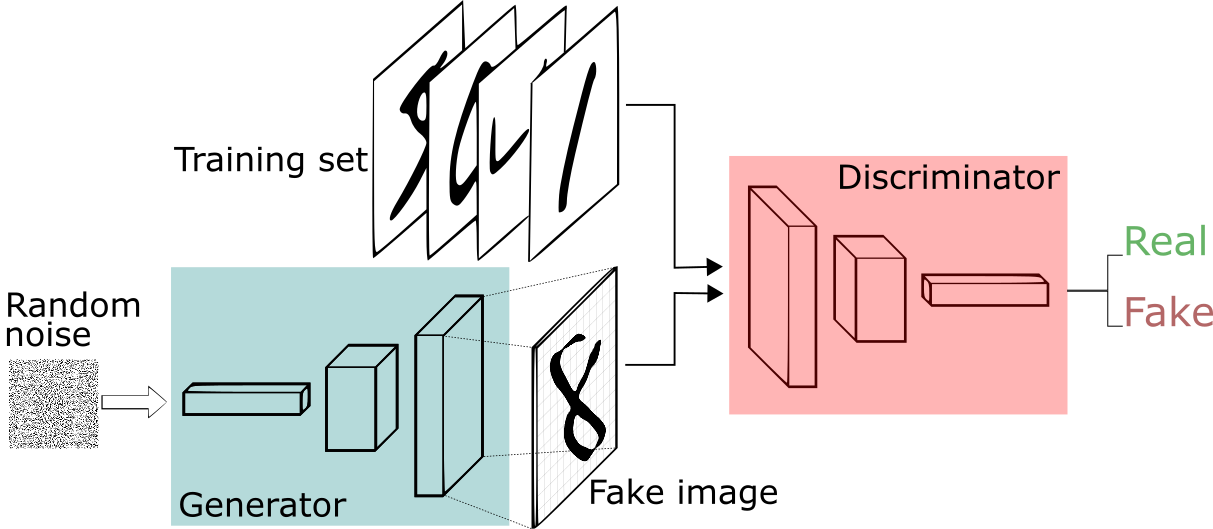
\includegraphics[scale=.25]{GANs.png}}
\caption{High-level overview of GANs}
\label{fig}
\end{figure}

In contrast, generative methods aim to predict features given a label rather than predicting a label given a set of features. As shown in figure 1, When two neural networks are combined to create a GAN, the generator neural network creates new data instances while the discriminator neural network assesses them for authenticity, determining whether or not each instance of data that it reviews belongs to the training dataset.

\subsection{Recurrent Neural Networks}

Artificial neural networks of the RNN variety can process sequential datasets. Each node's outputs can be utilized to impact its subsequent inputs, giving it the ability to behave in a temporally dynamic way. In contrast to conventional deep neural networks, which retain an independent link between inputs and outputs, recurrent neural networks' outputs are reliant on the prior input in the sequence. RNNS makes use of its capacity to retain the internal state of previous inputs to influence the subsequent input and output based on the previous input. This makes it suitable for both time series and datasets with sequences to predict the next output. However, because RNN networks only anticipate outputs based on the most recent inputs, they are not capable of memorizing input from a great distance.LSTM models are used to overcome this limitation.
\subsection{Long short-term Memory}

Long short-term memory networks, or LSTMs, are employed in deep learning. It is a kind of recurrent neural network (RNN) that has been capable of comprehending long-term relationships, particularly in sequence prediction tasks. Because of the endurance of human memory, new ideas can be processed without having to start over from scratch. Recurrent neural networks are able to address this, whereas traditional neural networks cannot. For persistence, they make use of loops. However, LSTM excels at handling long-term dependencies, whereas RNN does not. The idea was introduced by Hochreiter \& Schmidhuber in 1997.   In order to maintain information flow, LSTMs require a cell state, which has only a minor linear correlation. Gates are utilized to change the status of a cell's information. The amount to be sent through is decided by the gates using a sigmoid neural network and a point-wise multiplication operation. LSTMs also have similar chain-like structure, but the repeating module is built differently as shown in figure 2. There are four neural network layers instead of just one, and they interact in unique ways.
\begin{figure}
\centerline{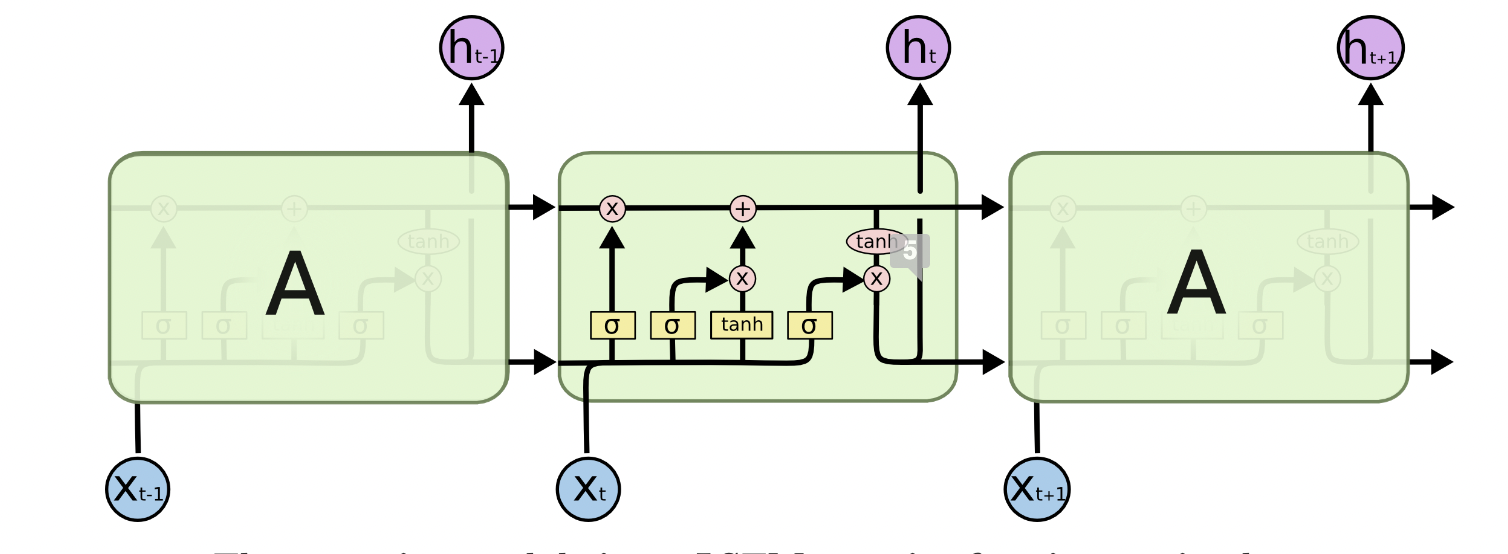
\includegraphics[scale=.25]{LSTM.png}}
\caption{The repeating module in an LSTM contains four interacting layers}
\label{fig}
\end{figure}

\subsection{Methodology}
The overall structure of our model can be explained in two sections
\begin{enumerate}
    \item Data Preprocessing
    \item Model Generation
\end{enumerate}

\subsubsection{Data Preprocessing}
Our experiments' dataset is GiantMIDI-Piano, a classical piano MIDI dataset containing 10,855 MIDI files of 2,786 composers. The data is stored as midi files. We use a python library called music21 to extract musical notes from midi files. At first, we will be pulling musical notes in alphabetical form from midi files and storing them in an array. We will be using a dictionary to map musical notation in alphabets to integers based on their pitch, and this newly created array will be normalized between a range of -1 and 1. The resulting list will be stored as a NumPy array.

\subsubsection{Model Generation}

Our model, inspired by MuseGAN from Hao-Wen Dong and colleagues, consists of two neural networks. A Generator and A Discriminator. To preserve the temporal relationship in musical data, we will implement a couple of RNN layers at the beginning of the network. Each generator and Discriminator consist of an LSTM followed by a Bi-Directional LSTM at the input. In Generator, LSTM layers are followed by three dense layers and in the Discriminator by two dense layers. Both use LeakyReLU activation. The output of the generator will be the shape of the input noise sequence. It is a dense layer with 'tanh' activation. Discriminator output consists of a dense layer with sigmoid activation. It is a binary output saying the input is real or fake. The figure 3 shows architecture of the proposed Generator network and figure 4 shows architecture of Discriminator

\begin{figure}
\centerline{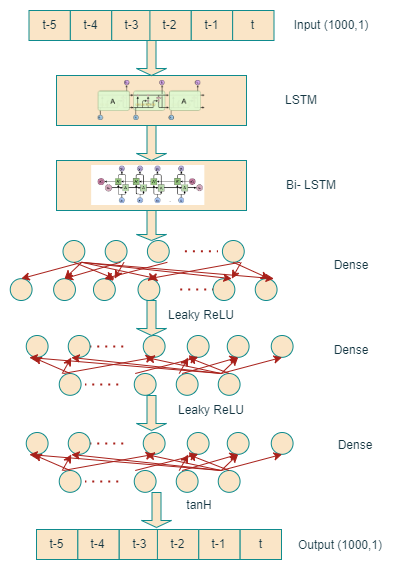
\includegraphics[scale=.4]{Generator.png}}
\caption{Architecture of Generator Network}
\label{fig}
\end{figure}

\begin{figure}
\centerline{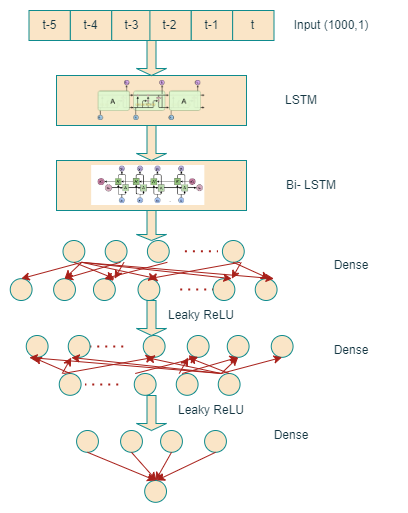
\includegraphics[scale=.4]{Discriminator.png}}
\caption{Architecture of Discriminator Network}
\label{fig}
\end{figure}

\section{Experimental Setup and Demonstration}
The project makes use of Giant MIDI Piano dataset \cite{b7}. The Standard MIDI File (SMF) is a file format that enables the MIDI protocol to be supported by electronic musical instruments, computers, and other devices. Electronic musical instruments and other devices may talk with one another and exchange data thanks to the MIDI (Musical Instrument Digital Interface) standard. SMFs are used to store and exchange music sequences, which include details on the notes, pitches, and durations of a song as well as different performance factors including velocity, pitch bend, and sustain pedal. Other information, such lyrics and metadata, can be found in SMFs.SMFs are frequently employed in a range of settings, including live performances, education, and music production. They are assisted by a wide range of hardware and software tools, such as sequencers, synthesisers, and digital audio workstations. GiantMIDIPiano dataset of 38,700,838 piano notes from 10,855 different, original classical piano pieces by 2,786 composers. GiantMIDI-Piano has a 1,237 hour running time. The chosen subset includes 1,787 composers' 24,253,495 piano notes from 7,236 different pieces. Utilizing meta-data from IMSLP, GiantMIDI-Piano transposes audio files from YouTube.


Python 3.8, a stable version, and Tensor flow 2.10.0 are both used in the project. TensorFlow python library is available for free and contributes to the development of efficient mathematical computations. As a result of its highly adaptable architecture, it can be seamlessly deployed across several platforms. CUDA 11.3 was used to use GPU for ML computing and it has smooth integration with python programming language. The project also made use of Ubuntu as the operating system because of various library dependencies. Azure ML – Standard NC6 VM with Nvidia Tesla K80 was used to train the huge dataset. By using CUDA for deep learning, ray tracing, crash simulations, energy exploration, and other applications, users may process data more quickly. For tightly connected parallel computing applications, the NC configuration offers a low latency, high-throughput network interface. The project makes use of two libraries Music 21 and midi2audio with the help of which midi file is converted into notes and vice versa and for converting midi to audio.

After data preprocessing, 35287752 sequences of 100 timesteps long music are generated. To get compatible with Tensorflow LSTM units and for better training performance, we limited our batch size to 128. During each epoch, 120 random sequences are extracted from the dataset. Random noises of batch size are generated and fed to the generator. The generator will generate a musical sequence from random noise. The discriminator is first trained with authentic music as a positive scenario, and discriminator\_real\_loss is calculated; then the same discriminator is trained against generated music as false music, and the discriminator\_fake\_loss is calculated. Discriminator loss will (discriminator\_real\_loss + discriminator\_fake\_loss )/2 . A combined model is created by combining the generator's output as the discriminator's input, and the model will be trained against generated sequence as a positive scenario. The integrated model's generator is trainable where the discriminator will not be. A High-level representation of the integrated model is shown in figure 5. 

\begin{figure}
\centerline{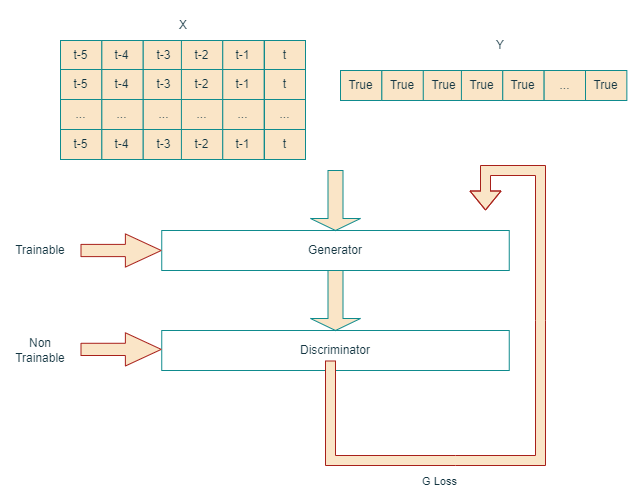
\includegraphics[scale=.4]{Combined.png}}
\caption{Architecture of Discriminator Network}
\label{fig}
\end{figure}

\section{Discussion}

The model was successfully able to combine the capabilities of LSTM and GAN to produce new music. The piano roll distribution for the generated music was different from the training data. But the piano roll distribution for newly generated music was having similar characteristics. We believe lack of dropout layer is the root cause of this behaviour. There is no standard evaluation criteria for music generated algorithm. So, there was no way to identify and distinguish between the output generated. That can also lead to such behaviour. We believe that implementing Wasserstein loss instead of binary cross entropy will generation music of distributed nature. Currently the model was trained for 100 epochs and the discriminator loss and generator loss started converging after 100 epochs. The figure 6 shows the same.

\section{Future Work}

We were able to develop a music generating model for this project with the help of GAN, LSTM, and recurrent neural networks operating on MIDI files. The produced model, which can produce both single-instrument and multi-instrument music, appears to have a lot of potential. The model can be enhanced, though, to produce better outcomes. The Giant MIDI Piano is the only dataset used to train the current music creation model, and the created music appears to have a similar tone. The model can be trained using other data sets, such as the Persian MIDI Dataset and Lakh MIDI Dataset, to produce music with a wider range of tones and greater originality. By feeding the model drum data  and multiple instrument chord to produce music with a range of varied intensities, further advancements can be realized.Creating a user interface for mobile or desktop for music creation can  provide better user experience. Since there isn't currently an evaluation matrix accessible to assess the output's quality and uniqueness, one needs to be created in order to compare how outstanding the new music is.

\section{Conclusion}
The project is an extension of the current musicGan model. The existing model which generates music using a GAN, does not take the relationship between the nodes of subsequent music into account. The music notes depend on the previous music notes because they are sequential data. We discover that recurrent neural networks are capable of inferring patterns from temporal data. The proposed approach uses LSTM and GAN neural networks  and was able to produce music that appears to have been written by a human. These two models were trained and was able to create whole new MIDI files by treating the notes and chords present in MIDI files as discrete sequential data. If we train the model by making adjustments to the training parameters , we anticipate that the results will be better. 
The model has an inherent limitations of the GiantPiano dataset we have used.  GiantMIDI-Piano does not provide beats, time signatures, key signatures, or scores. Additionally, there are no pitch spellings to distinguish between enharmonic sounds. The music score and the pianists' expressive performances are not separate in GiantMIDI-Piano. As the number of epochs reaches a certain limit the model faced overfitting issues due to the lack of randomness in the input music dataset. 

\begin{figure}
\centerline{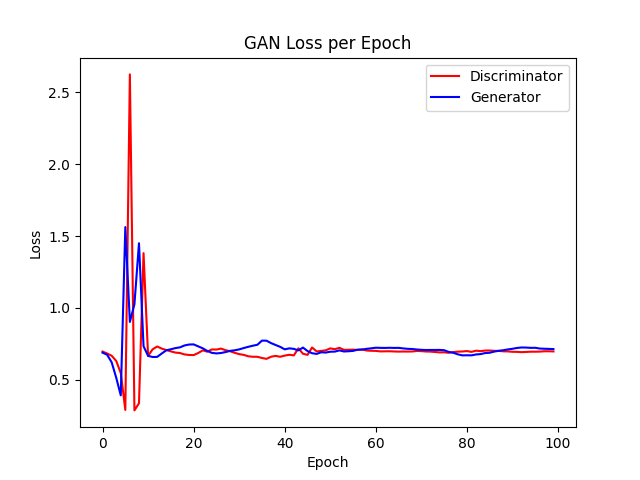
\includegraphics[scale=.4]{GAN_Loss_per_Epoch_final .png}}
\caption{GAN loss per epoch}
\label{fig}
\end{figure}

\begin{thebibliography}{9}

    \bibitem[1]{b2} Hao-Wen Dong, Wen-Yi Hsiao, Li-Chia Yang, Yi-Hsuan Yang. (2018). MuseGAN: Multi-track Sequential Generative AdversarialNetworks for Symbolic Music Generation and Accompaniment.
    \href{https://dblp.uni-trier.de/db/conf/aaai/aaai2018.htmlDongHYY18}{National Conference on Artificial Intelligence, 32(1), 34–41}

    \bibitem [2]{b1} Hao-Wen Dong, Yi-Hsuan Yang. (2018b). Convolutional Generative Adversarial Networks with Binary Neurons for Polyphonic MusicGeneration.
    \href{https://arxiv.org/pdf/1804.09399}{ArXiv: Learning}

  \bibitem [3]{b4}Brunner, G., Wang, Y., Wattenhofer, R., Wiesendanger, J. (2017). JamBot: Music Theory Aware Chord Based Generation of Polyphonic Music with LSTMs
    \href{https://doi.org/10.1109/ictai.2017.00085}{2017 IEEE 29th International Conference on Tools With Artificial Intelligence (ICTAI)}
    
    \bibitem [4]{b3} Sajad, S., Dharshika, S., Meleet, M.(2021). Music Generation for Novices Using Recurrent Neural Network (RNN).
    \href{https://doi.org/10.1109/icses52305.2021.9633906}{2021 International Conference on Innovative Computing, Intelligent Communication and Smart Electrical Systems (ICSES)}
    
  
    \bibitem [5]{b5}Alex Graves. (2013). Generating Sequences With Recurrent Neural Networks.

    \bibitem [6]{b6}Schmidhuber, J. (2002). Finding temporal structure in music: blues improvisation with LSTM recurrent networks.
    \href{https://doi.org/10.1109/nnsp.2002.1030094}{ Proceedings of the 12th IEEE Workshop on Neural Networks for Signal Processing.}
    
    \bibitem [7]{b7}Kong, Q., Li, B., Chen, J., and Wang, Y. (2022). GiantMIDI-Piano: A Large-Scale MIDI Dataset for Classical Piano Music.
    \href{https://doi.org/10.5334/tismir.80}{Transactions of the International Society for Music Information Retrieval, 5(1), 87–98.}
    
\end{thebibliography}

\end{document}
